\documentclass[]{report}
\usepackage{lscape}
\usepackage[utf8]{inputenc}
\usepackage[spanish]{babel}
\usepackage{graphicx}
\usepackage{subfigure}
% Title Page
\title{}
\author{}


\begin{document}
\maketitle
%\begin{landscape}
	\begin{table}[h!]
	\centering
	\begin{tabular}{|c|c|c|c|c|c|c|c|c||}
	 
%	& \multicolumn{3}{c}{Matlab} 
%	& &  \multicolumn{2}{ c| }{QGround}\\ \cline{2-7}
	
	\cline{1-7}
	&  \multicolumn{2}{ c| }{T. Proc}
	&  \multicolumn{2}{ c| }{Costo estimado}
	&  \multicolumn{2}{c|}{Costo en simulación}\\
	\cline{2-7}
	
	\multicolumn{1}{ |c| }{Polígono}
	& \multicolumn{1}{ |c| }{Torres}
	&  \multicolumn{1}{ c| }{Vasquez}
	& \multicolumn{1}{ c| }{Torres}
	& \multicolumn{1}{ c| }{Vasquez}
	& \multicolumn{1}{ c| }{Torres}
	& \multicolumn{1}{ c| }{Vasquez}\\
	
	
	\hline
	Path\_1  & 0.0016 & 0.0047 & 85.3847  & 78.55 & 95 &    85\\ 
	Path\_2  & 0.0027 & 0.0066 & 189.3541 & 186.2209 & 201 &198 \\ 
	Path\_3  & 0.0021 & 0.0064 & 125.9197 & 119.2976 & 130  &126 \\ 
	
	Path\_4  & 0.0024  & 0.0064 & 178.478 & 173.8069 & 187 & 180\\ 
	Path\_5  & 0.0012 & 0.0075 & 141.5335 & 138.3032 & 150 & 146\\ 
	Path\_6  & 0.0023 & 0.0077 & 167.1019 & 164.53 & 174 & 166 \\ 
	\hline
\end{tabular} 
\caption{Cuadro comparativo del costo y el tiempo de procesamiento de cada polígono. Del \textit{Path\_1} al \textit{Path\_3} regresan al punto inicial y del \textit{Path\_4} al \textit{Path\_6} terminan en un punto diferente.}
\label{table}
\end{table}

\section{Rutas y polígonos}

%\rotatebox[origin=c]{-90}{same_ji_1.eps}
%--------------Path_1-----
\begin{figure}%
	
	\centering
	\subfigure[][]{%
		\label{same_ji_1}%
		\rotatebox[origin=c]{-90}{\scalebox{-1}[1]{ 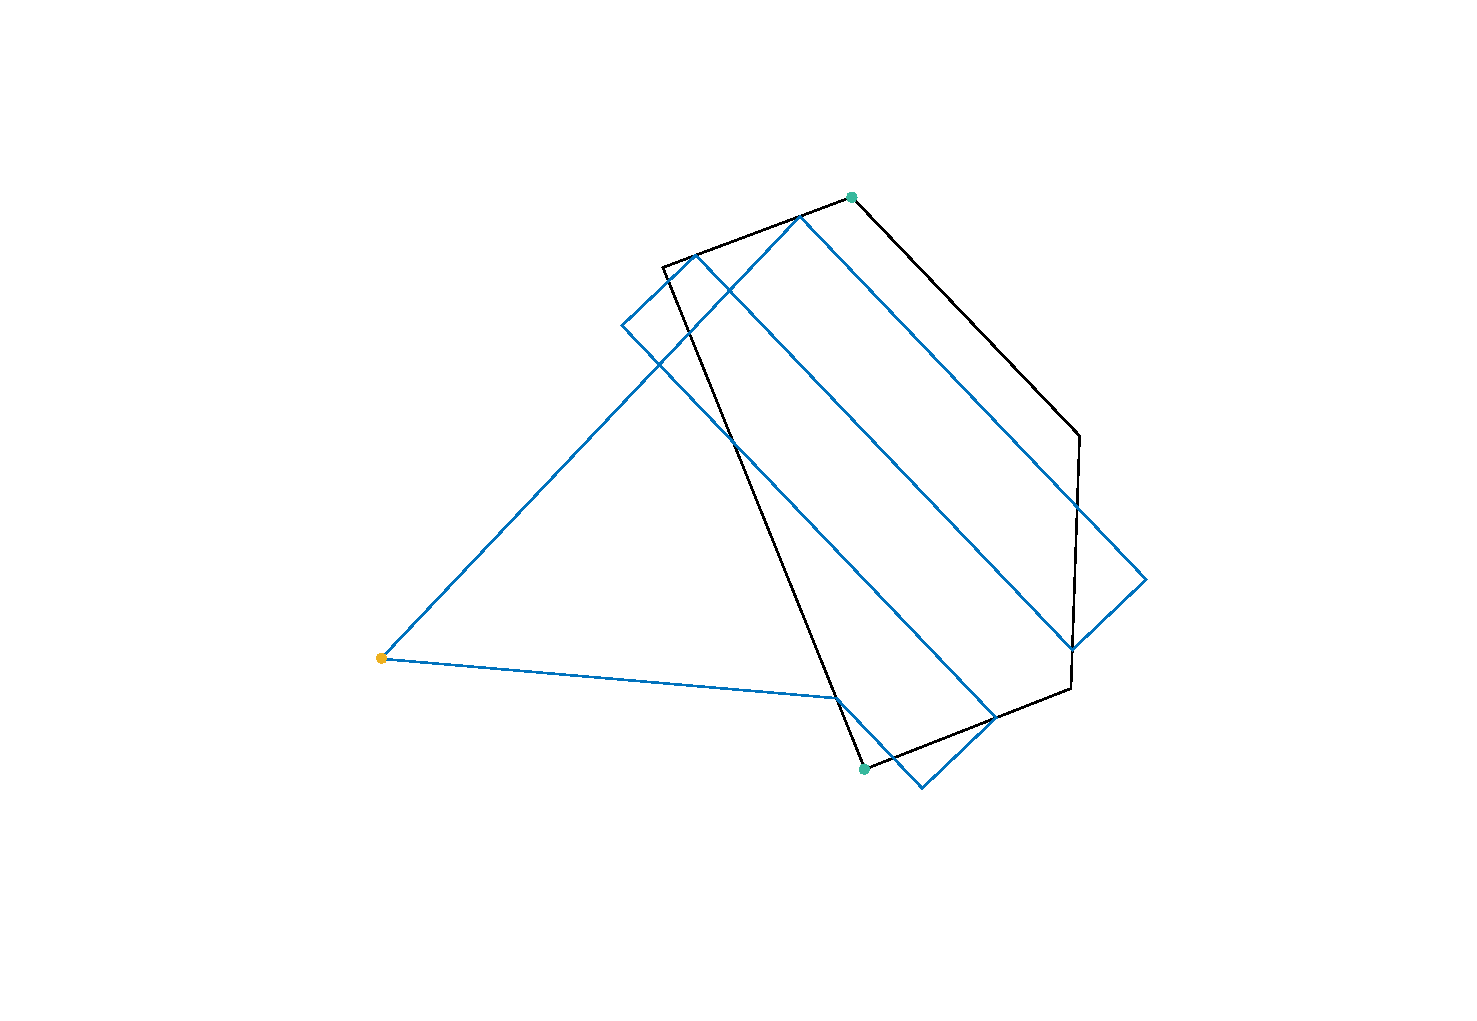
\includegraphics[height=4cm]{same_ji_1_1.eps}}}}%
		\hspace{8pt}%
	\subfigure[][]{%
		\label{same_ji_sim_1}%
		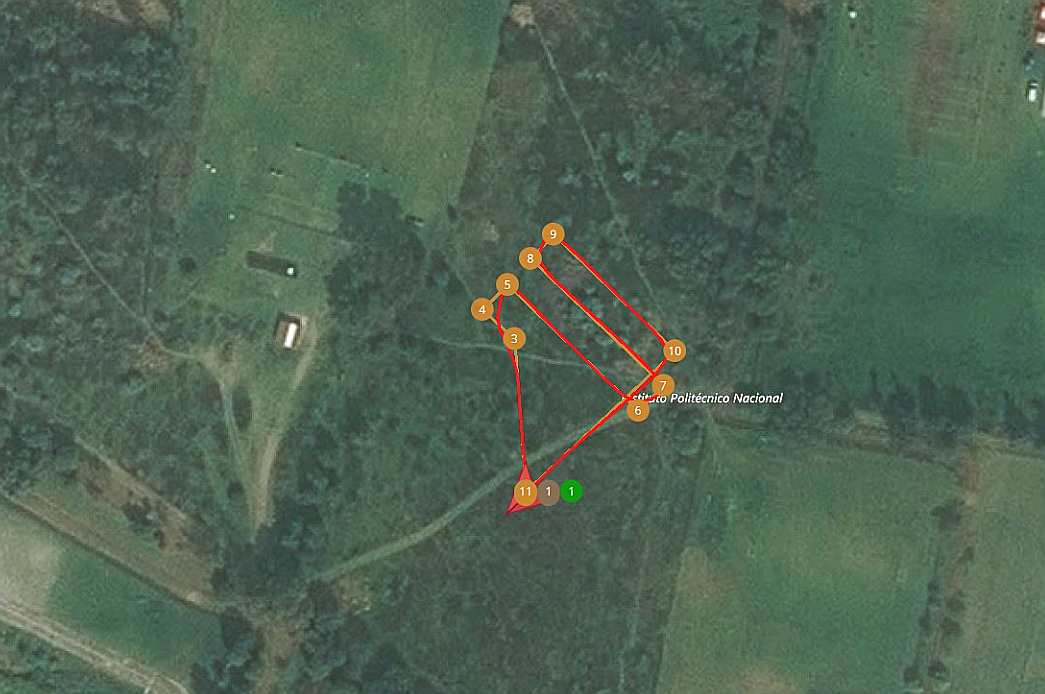
\includegraphics[height=3.5cm]{same_ji_1.png}} \\
	\subfigure[][]{%
		\label{same_torres_1}%
		\rotatebox[origin=c]{-90}{\scalebox{-1}[1]{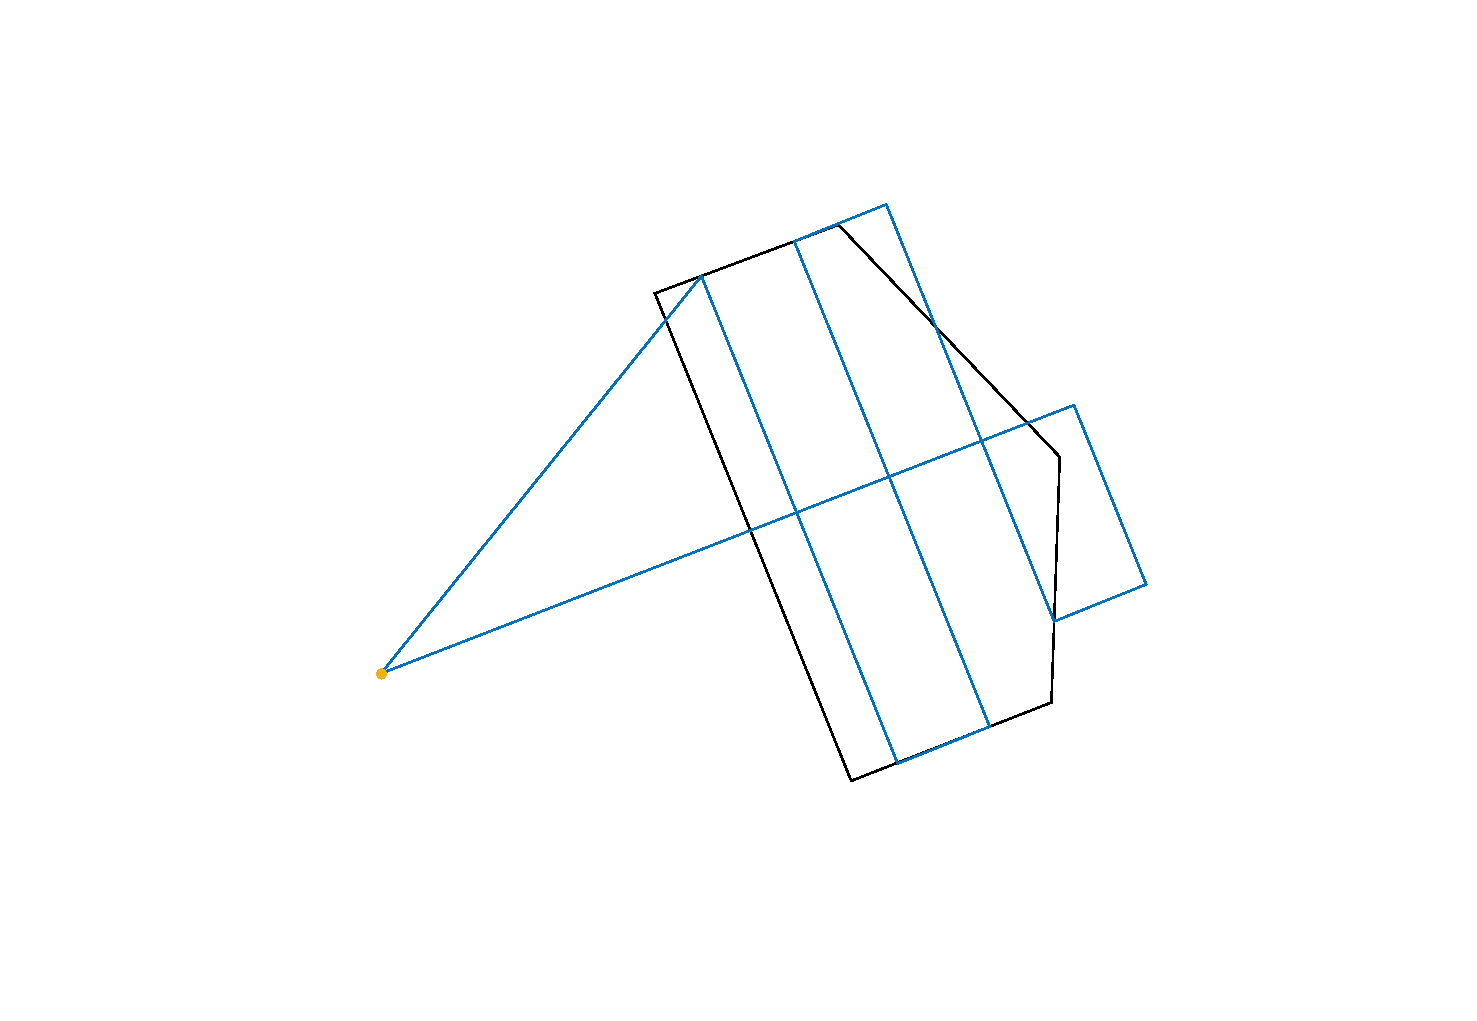
\includegraphics[height=4cm]{same_torres_1_1.eps}}}}%
	\hspace{8pt}%
	\subfigure[][]{%
		\label{same_torres_sim_1}%
		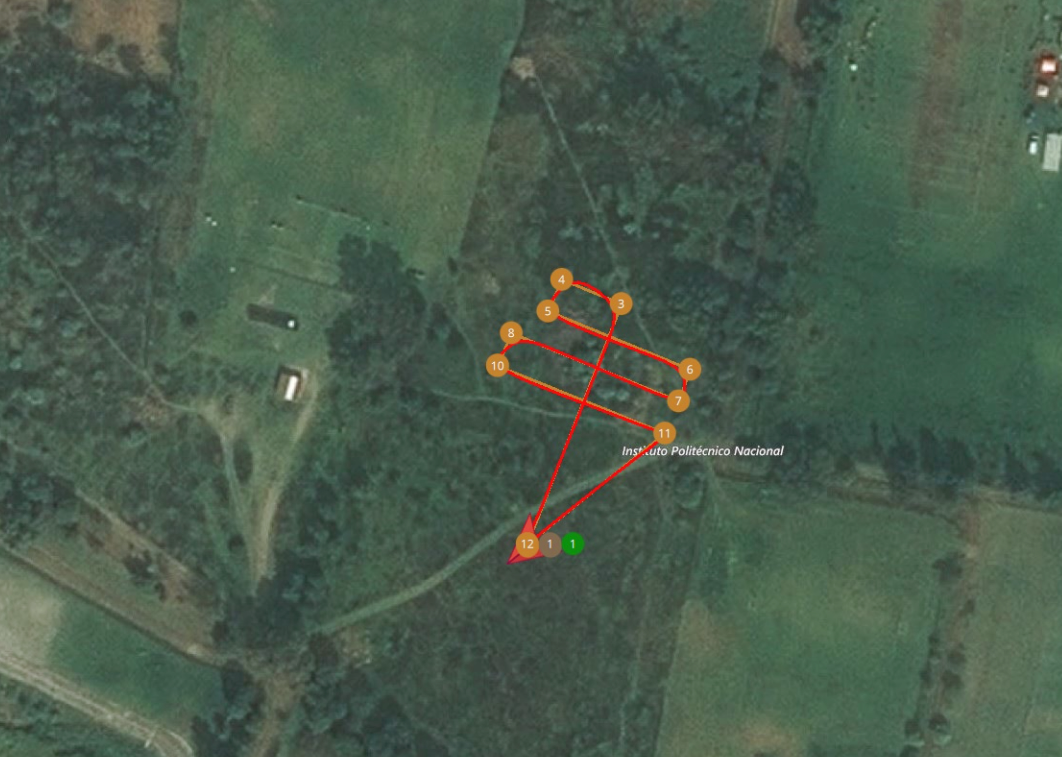
\includegraphics[height=3.5cm]{same_torres_1.png}}%
	\caption[A set of four subfigures.]{Polígono y ruta uno:}
		\subref{same_ji_1} Ruta y polígono para el \textit{Path\_1} (Vasquez);
		\subref{same_ji_sim_1} simulación para el \textit{Path\_1} (Vasquez);
		\subref{same_torres_1} ruta y poligono para el \textit{Path\_1} (Torres); y,
		\subref{same_torres_sim_1} simulación del \textit{Path\_1.} (Torres)%
	\label{path_1}%
\end{figure}
%-----------


%--------
%----Path_2
\begin{figure}%
	\centering
	\subfigure[][]{%
		\label{same_ji_2}%
		\rotatebox[origin=c]{-90}{\scalebox{-1}[1]{ 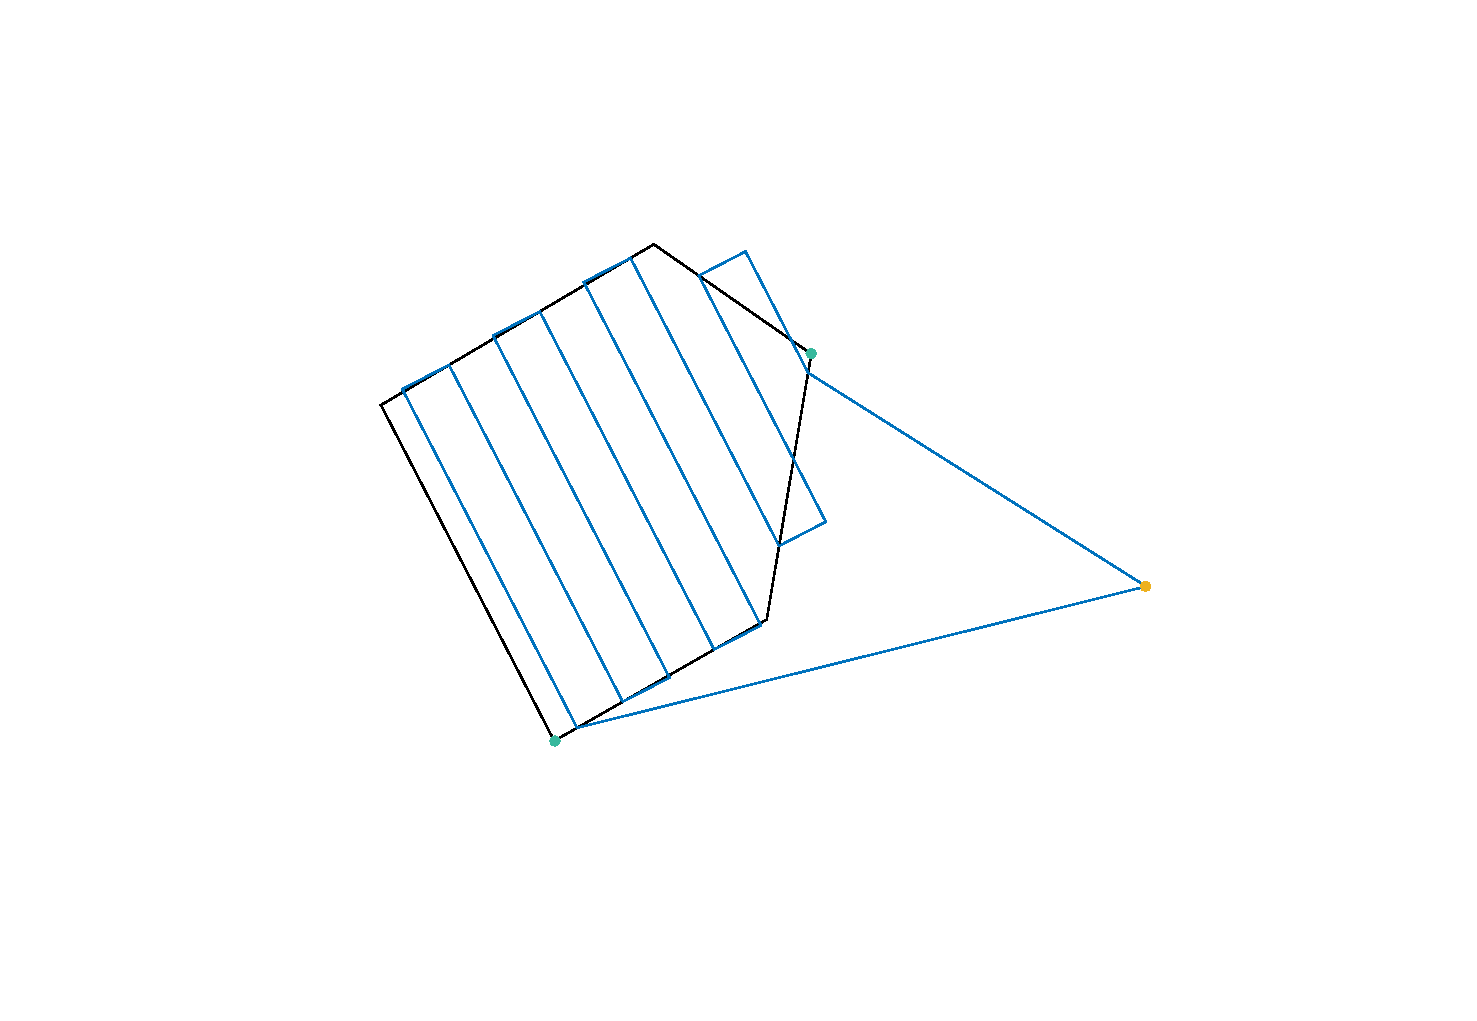
\includegraphics[height=4cm]{same_ji_2_1.eps}}}}%
	\hspace{8pt}%
	\subfigure[][]{%
		\label{same_ji_sim_2}%
		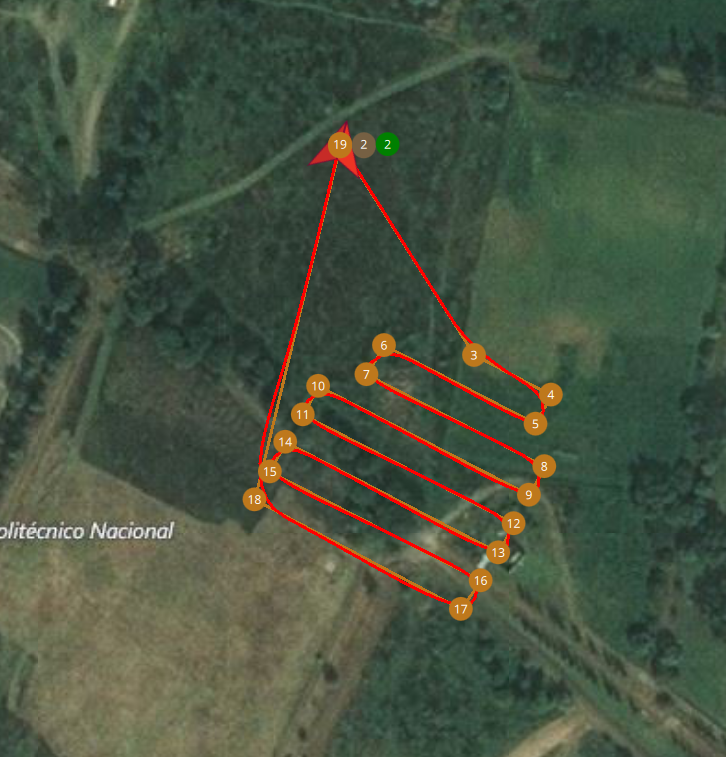
\includegraphics[height=3.5cm]{same_2_ji.png}} \\
	\subfigure[][]{%
		\label{same_torres_2}%
		\rotatebox[origin=c]{-90}{\scalebox{-1}[1]{ 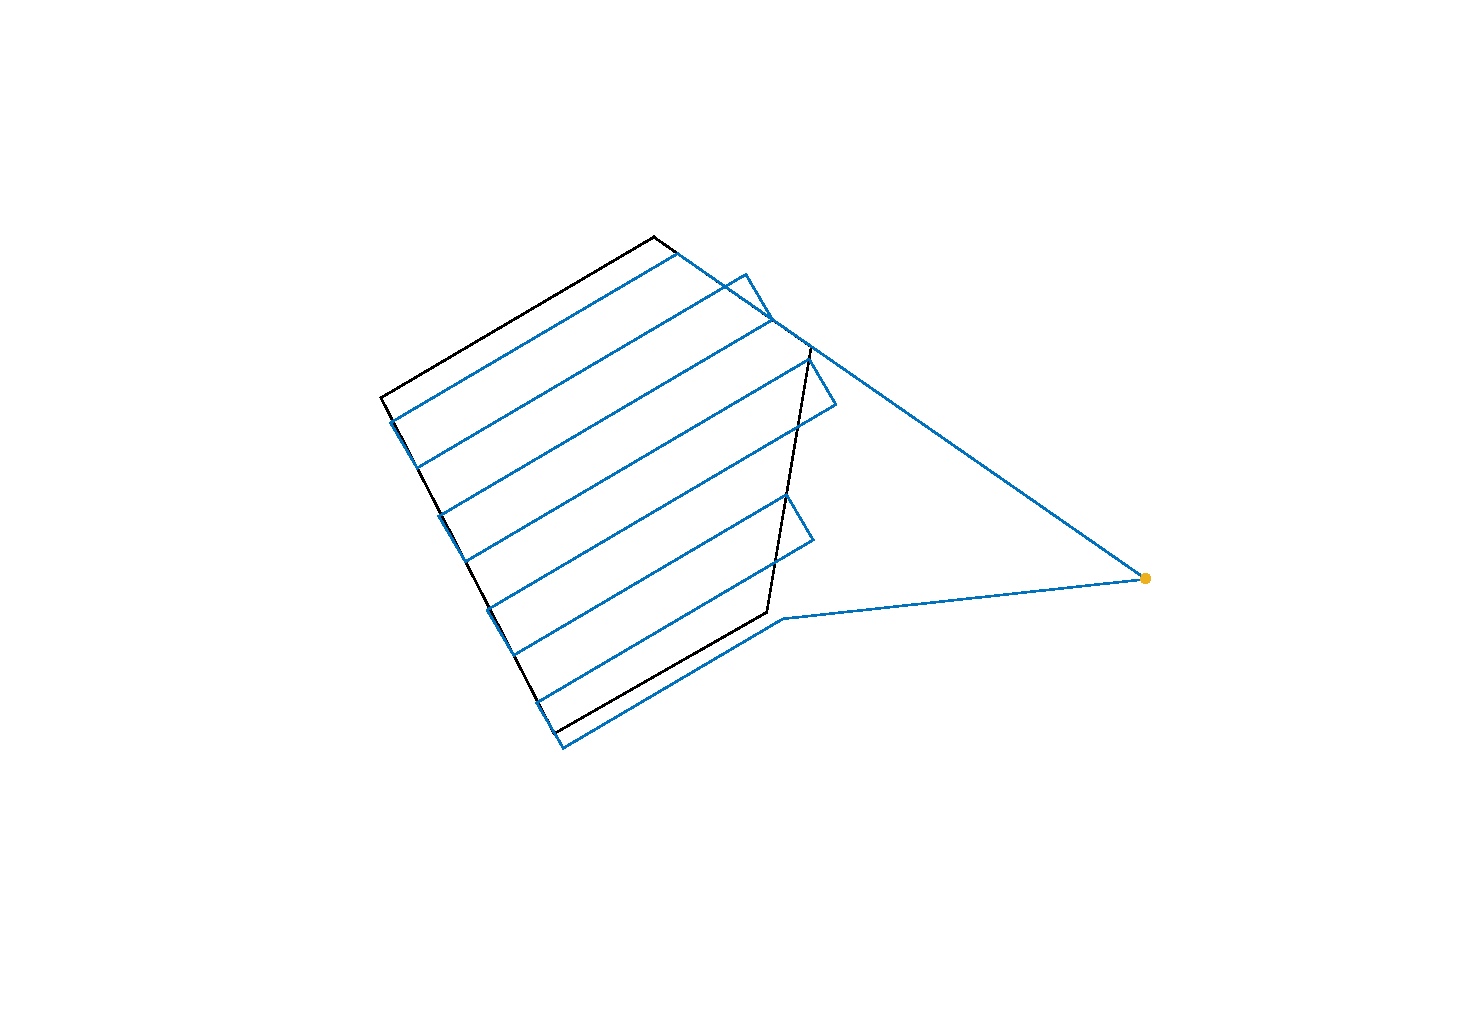
\includegraphics[height=4cm]{same_torres_2_1.eps}}}}%
	\hspace{8pt}%
	\subfigure[][]{%
		\label{same_torres_sim_2}%
		
		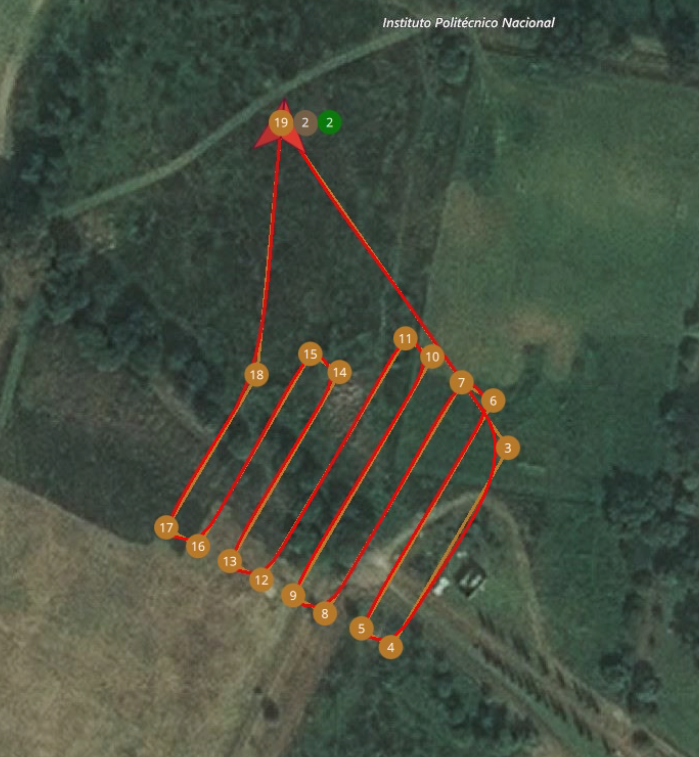
\includegraphics[height=3.5cm]{same_2_torres.png}}%
	\caption[A set of four subfigures.]{Polígono y ruta dos:}
	\subref{same_ji_2} Ruta y polígono para el \textit{Path\_2} (Vasquez);
	\subref{same_ji_sim_2} simulación para el \textit{Path\_2} (Vasquez);
	\subref{same_torres_2} ruta y poligono para el \textit{Path\_2} (Torres); y,
	\subref{same_torres_sim_2} simulación del \textit{Path\_2.} (Torres)%
	\label{path_2}%
\end{figure}

%---Path_3----
\begin{figure}%
	\centering
	\subfigure[][]{%
		\label{same_ji_3}%
		\rotatebox[origin=c]{-90}{\scalebox{-1}[1]{ 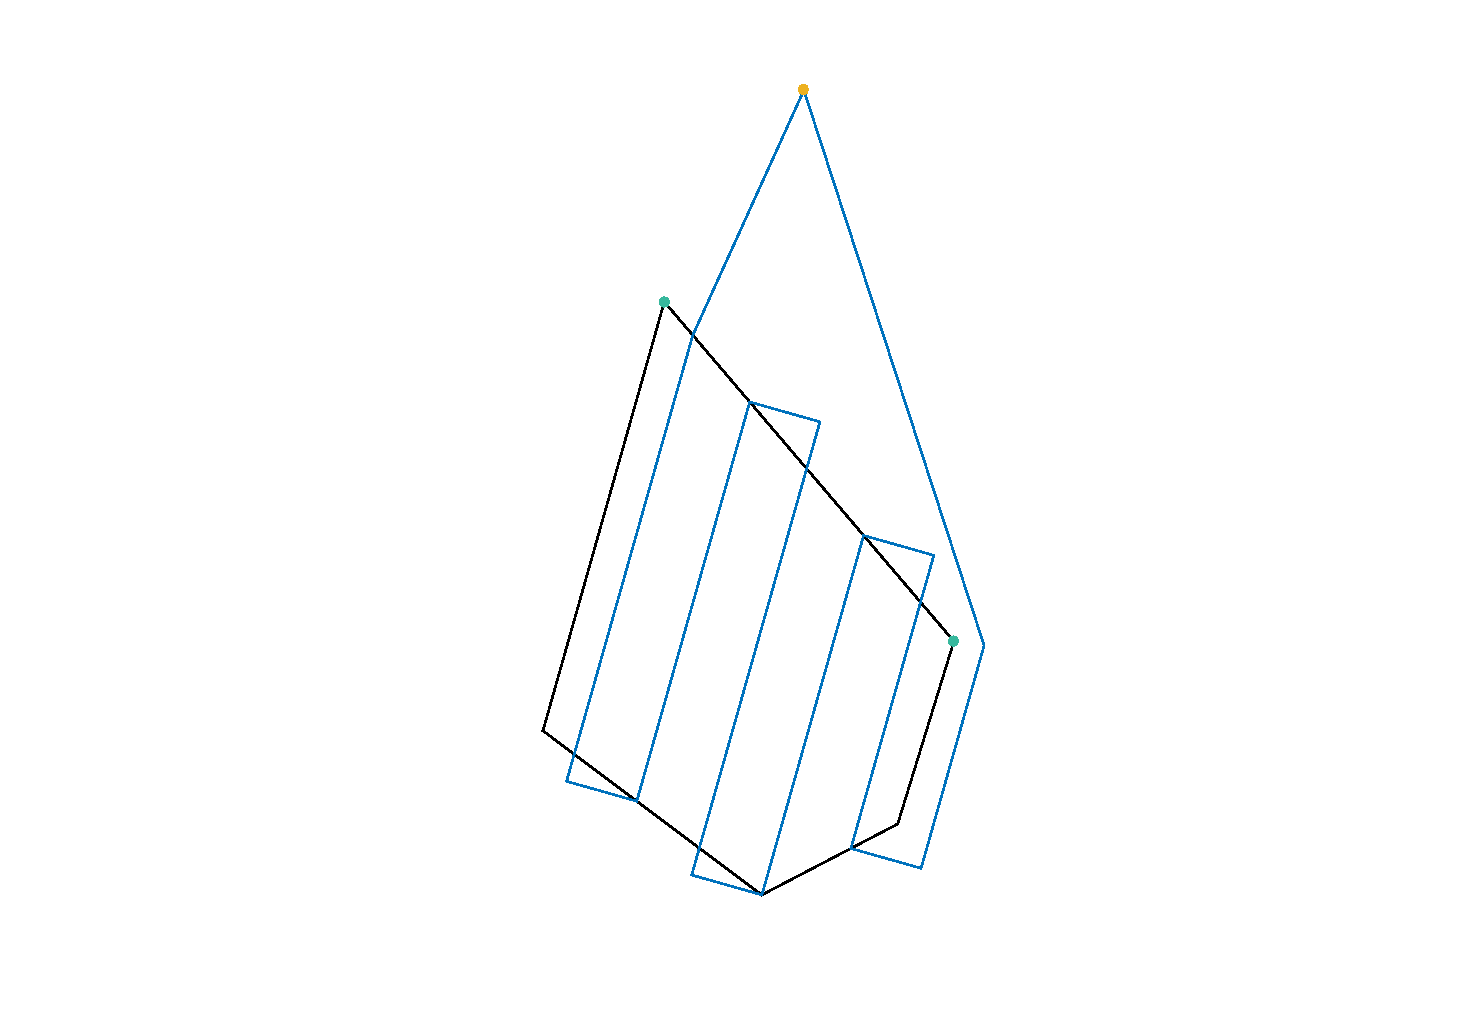
\includegraphics[height=4cm]{same_ji_3_1.eps}}}}%
	\hspace{8pt}%
	\subfigure[][]{%
		\label{same_ji_sim_3}%
		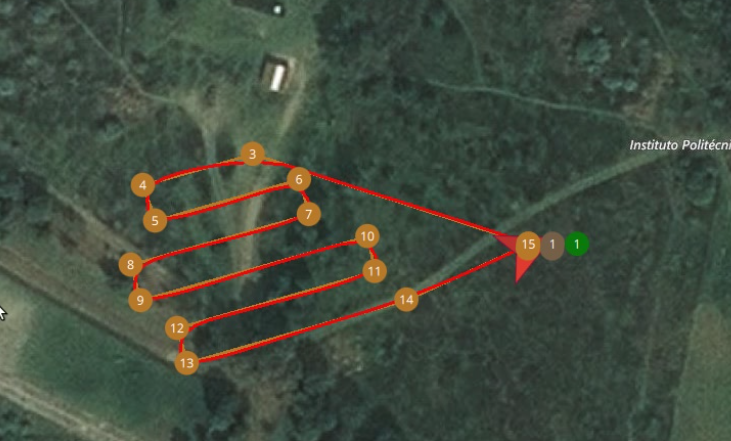
\includegraphics[height=3.5cm]{same_3_ji.png}} \\
	\subfigure[][]{%
		\label{same_torres_3}%
		\rotatebox[origin=c]{-90}{\scalebox{-1}[1]{ 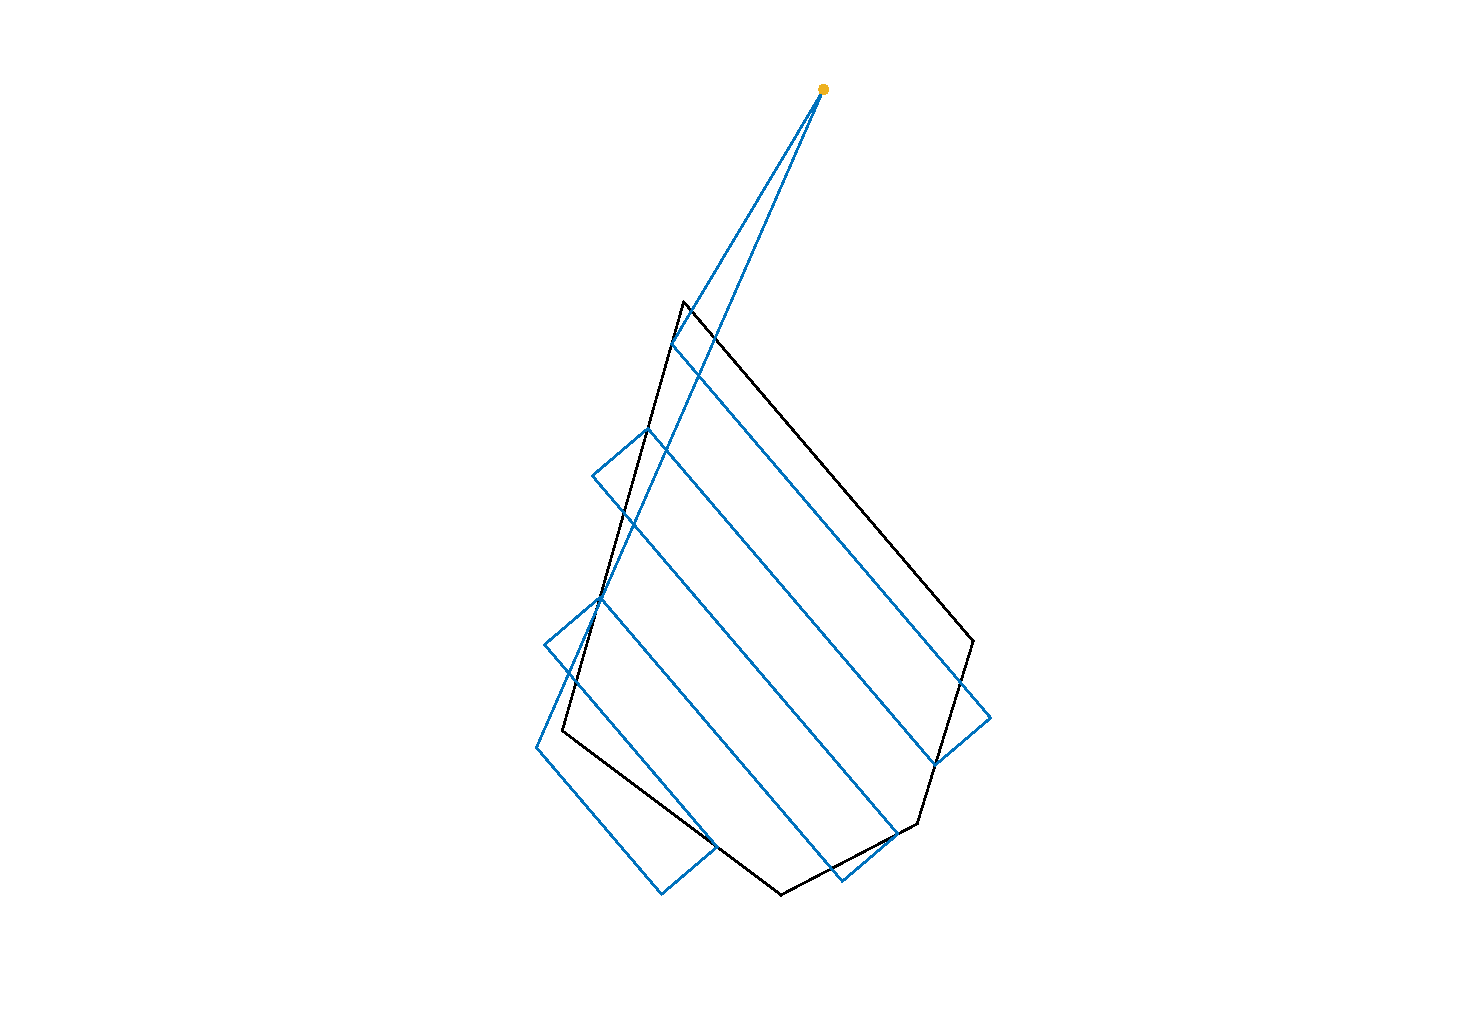
\includegraphics[height=4cm]{same_torres_3_1.eps}}}}%
	\hspace{8pt}%
	\subfigure[][]{%
		\label{same_torres_sim_3}%
		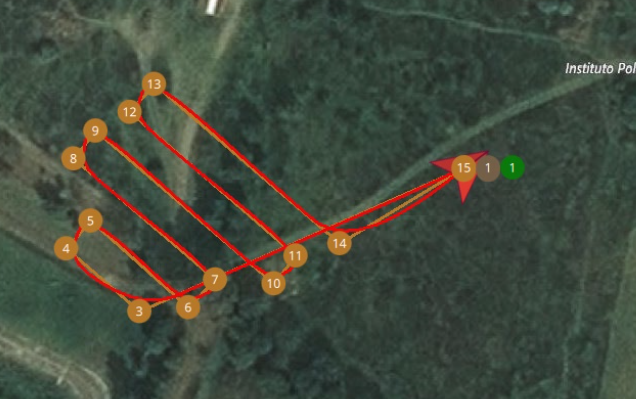
\includegraphics[height=3.5cm]{same_3_torres.png}}%
	
	\caption[A set of four subfigures.]{Polígono y ruta tres:}
	\subref{same_ji_3} Ruta y polígono para el \textit{Path\_1} (Vasquez);
	\subref{same_ji_sim_3} simulación para el \textit{Path\_3} (Vasquez);
	\subref{same_torres_3} ruta y poligono para el \textit{Path\_3} (Torres); y,
	\subref{same_torres_sim_3} simulación del \textit{Path\_3} (Torres)%
	\label{path_3}%
\end{figure}

%----Path_4----
\begin{figure}%
	\centering
	\subfigure[][]{%
		\label{same_ji_4}%
		\rotatebox[origin=c]{-90}{\scalebox{-1}[1]{ 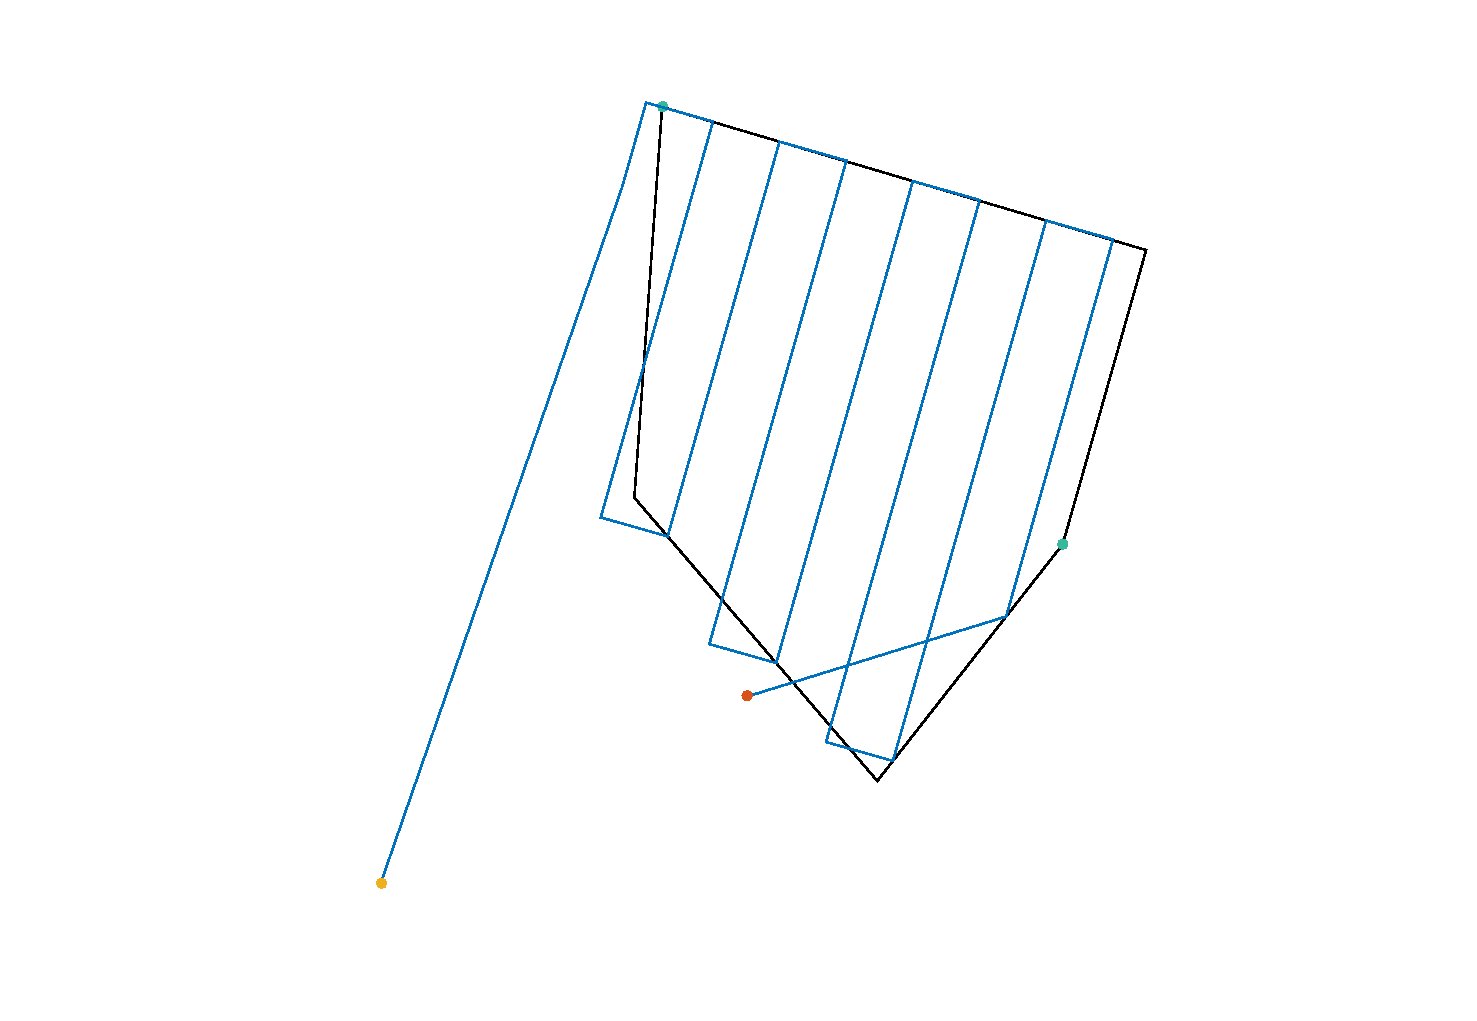
\includegraphics[height=4cm]{dif_ji_1_1.eps}}}}%
	\hspace{8pt}%
	\subfigure[][]{%
		\label{same_ji_sim_4}%
		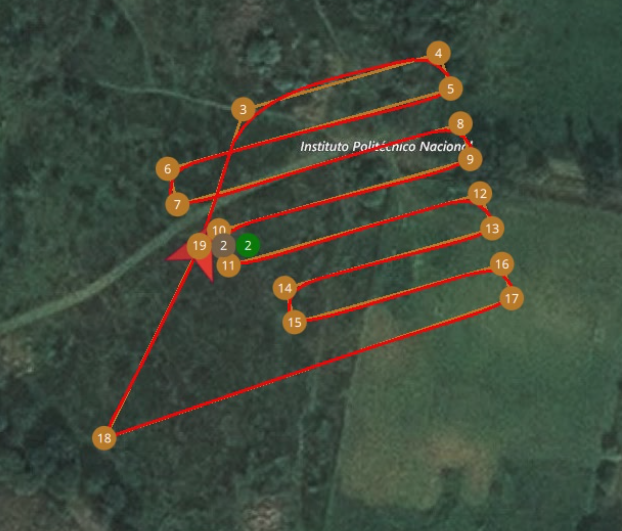
\includegraphics[height=3.5cm]{dif_1_ji.png}} \\
	\subfigure[][]{%
		\label{same_torres_4}%
		\rotatebox[origin=c]{-90}{\scalebox{-1}[1]{ 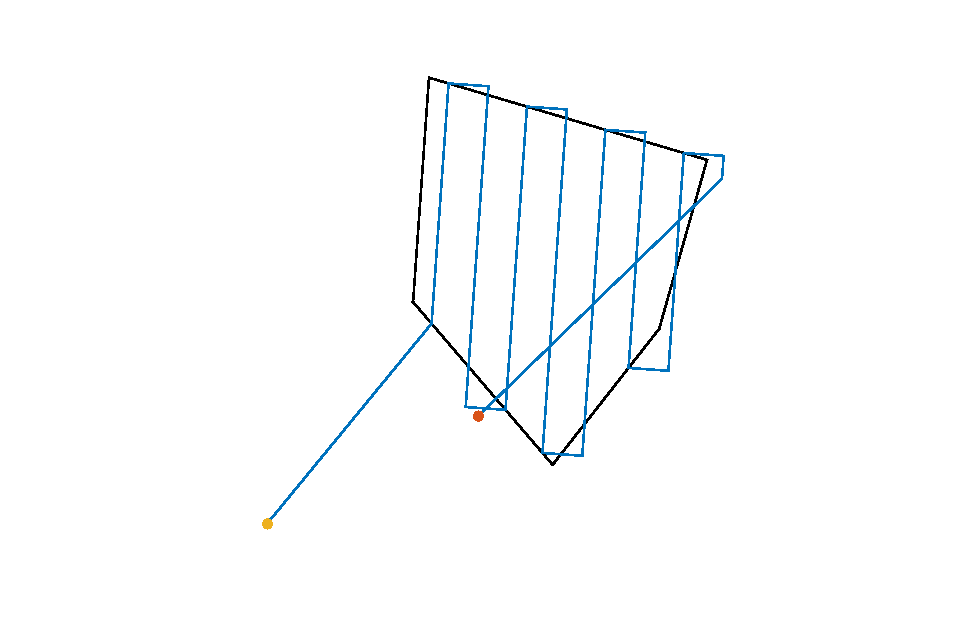
\includegraphics[height=4cm]{dif_torres_1_1.eps}}}}%
	\hspace{8pt}%
	\subfigure[][]{%
		\label{same_torres_sim_4}%
		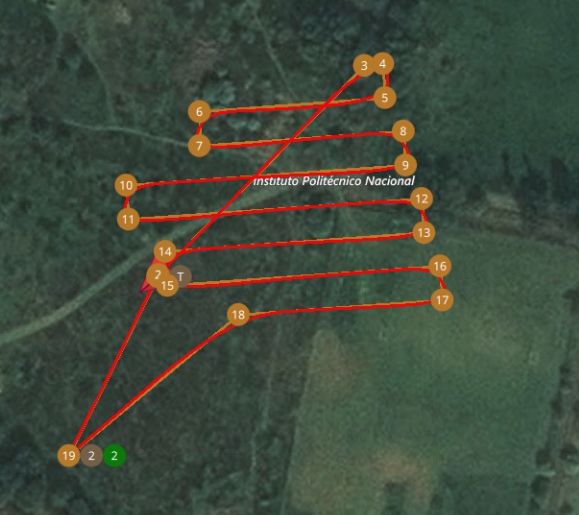
\includegraphics[height=3.5cm]{dif_1_torres.png}}%
	
	\caption[A set of four subfigures.]{Polígono y ruta cuatro:}
	\subref{same_ji_4} Ruta y polígono para el \textit{Path\_1} (Vasquez);
	\subref{same_ji_sim_4} simulación para el \textit{Path\_4} (Vasquez);
	\subref{same_torres_4} ruta y polígono para el \textit{Path\_4} (Torres); y,
	\subref{same_torres_sim_4} simulación del \textit{Path\_4} (Torres)%
	\label{path_4}%
\end{figure}


%----Path_5------
\begin{figure}%
	\centering
	\subfigure[][]{%
		\label{same_ji_5}%
		\rotatebox[origin=c]{-90}{\scalebox{-1}[1]{ 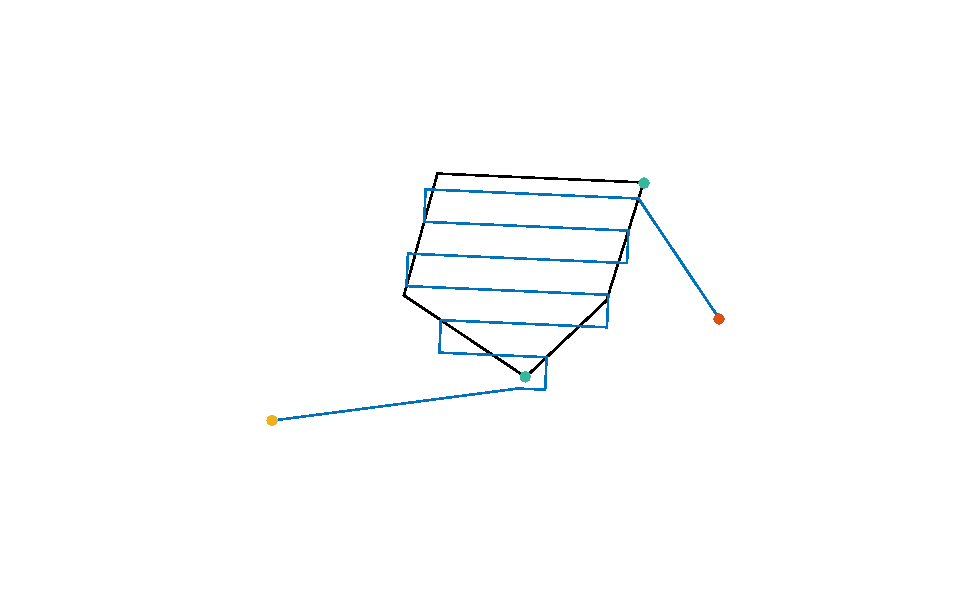
\includegraphics[height=4cm]{dif_ji_2_1.eps}}}}%
	\hspace{8pt}%
	\subfigure[][]{%
		\label{same_ji_sim_5}%
		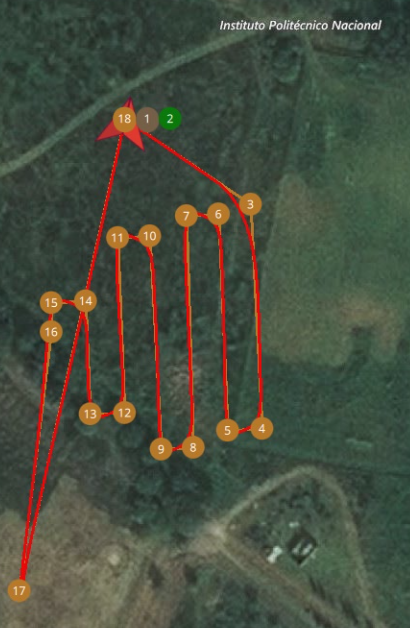
\includegraphics[height=3.5cm]{dif_2_ji.png}} \\
	\subfigure[][]{%
		\label{same_torres_5}%
		\rotatebox[origin=c]{-90}{\scalebox{-1}[1]{ 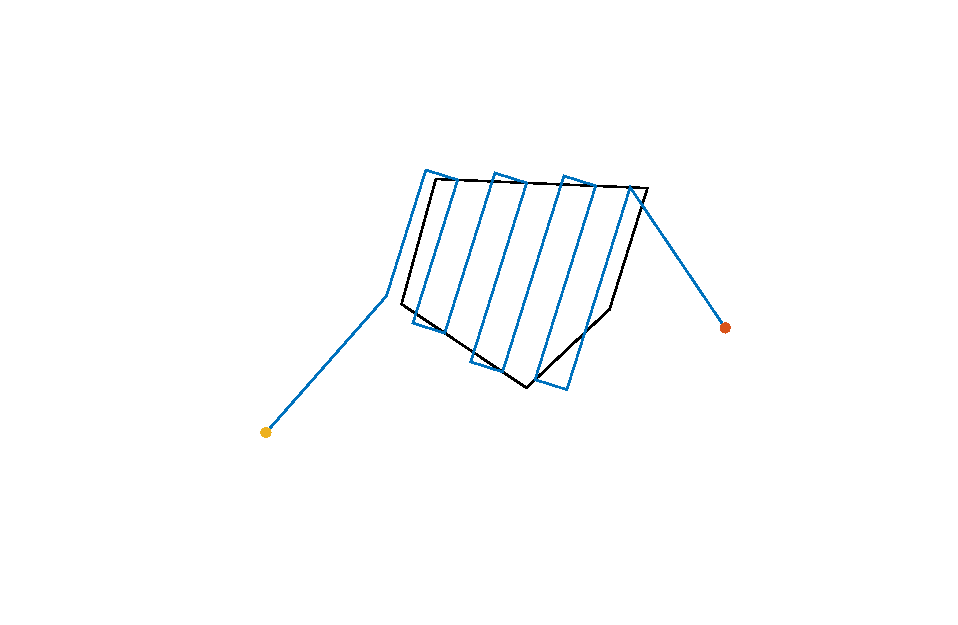
\includegraphics[height=4cm]{dif_torres_2_1.eps}}}}%
	\hspace{8pt}%
	\subfigure[][]{%
		\label{same_torres_sim_5}%
		
		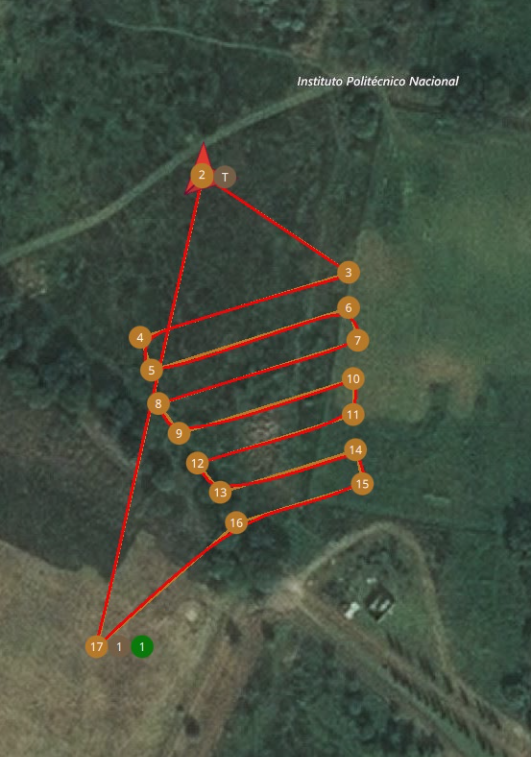
\includegraphics[height=3.5cm]{dif_2_torres.png}}%
	\caption[A set of four subfigures.]{Polígono y ruta cinco:}
	\subref{same_ji_5} Ruta y polígono para el \textit{Path\_5} (Vasquez);
	\subref{same_ji_sim_5} simulación para el \textit{Path\_5} (Vasquez);
	\subref{same_torres_5} ruta y poligono para el \textit{Path\_5} (Torres); y,
	\subref{same_torres_sim_5} simulación del \textit{Path\_5.} (Torres)%
	\label{path_5}%
\end{figure}

%----Path_5----------
\begin{figure}%
	\centering
	\subfigure[][]{%
		\label{same_ji_6}%
		\rotatebox[origin=c]{-90}{\scalebox{-1}[1]{ 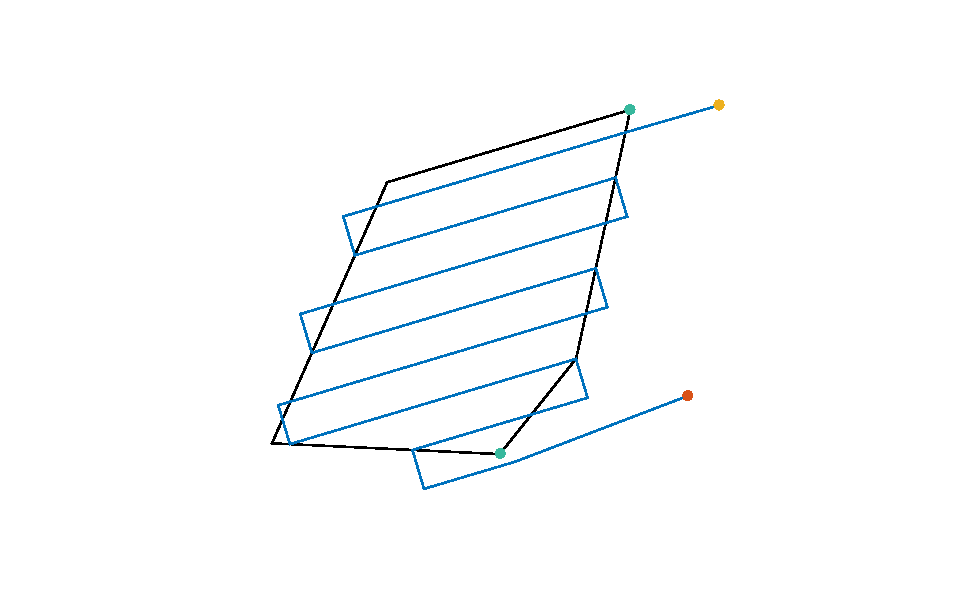
\includegraphics[height=4cm]{dif_ji_3_1.eps}}}}%
	\hspace{8pt}%
	\subfigure[][]{%
		\label{same_ji_sim_6}%
		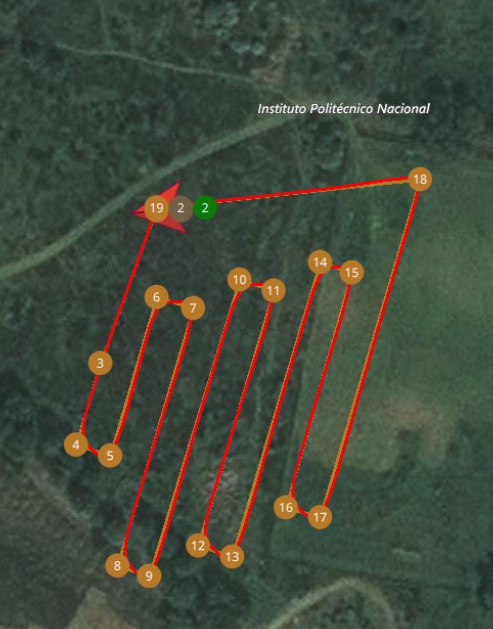
\includegraphics[height=3.5cm]{dif_3_ji.png}} \\
	\subfigure[][]{%
		\label{same_torres_6}%
		\rotatebox[origin=c]{-90}{\scalebox{-1}[1]{ 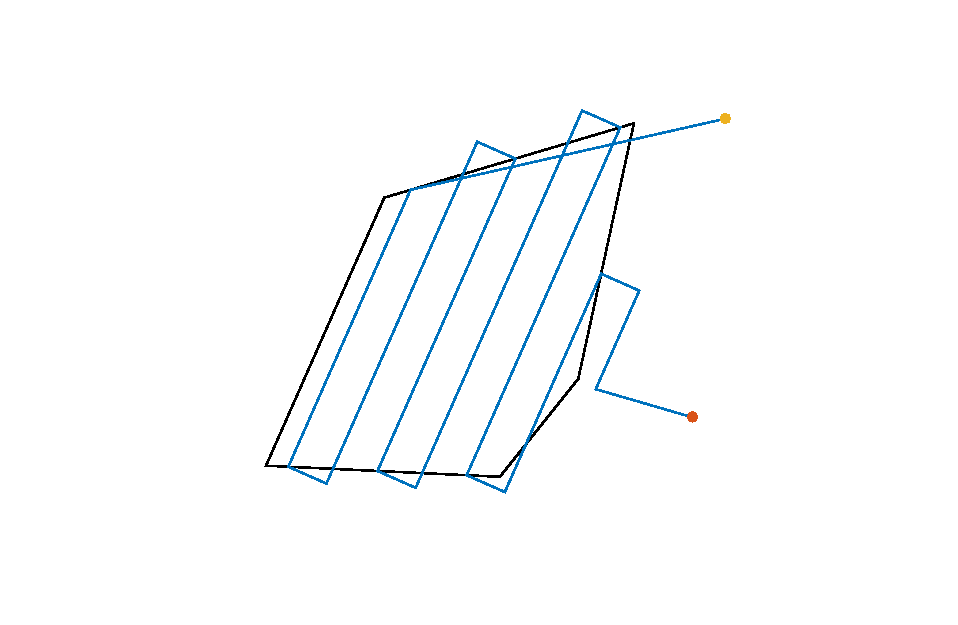
\includegraphics[height=4cm]{dif_torres_3_1.eps}}}}%
	\hspace{8pt}%
	\subfigure[][]{%
		\label{same_torres_sim_6}%
		
		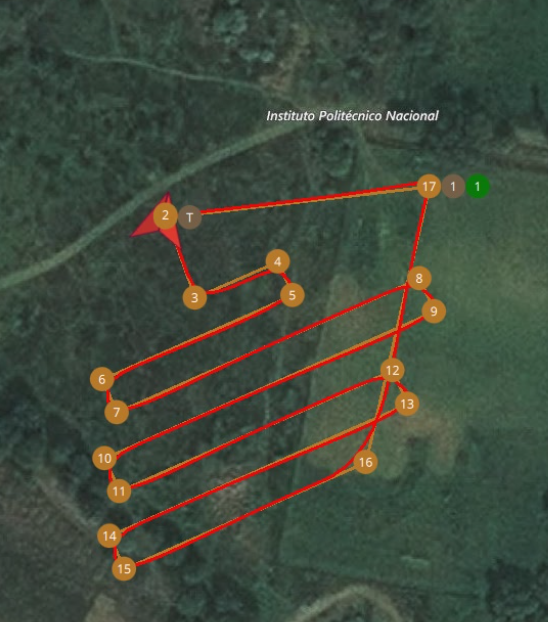
\includegraphics[height=3.5cm]{dif_3_torres.png}}%
	\caption[A set of four subfigures.]{Polígono y ruta seis:}
	\subref{same_ji_6} Ruta y polígono para el \textit{Path\_6} (Vasquez);
	\subref{same_ji_sim_6} simulación para el \textit{Path\_6} (Vasquez);
	\subref{same_torres_6} ruta y polígono para el \textit{Path\_6} (Torres); y,
	\subref{same_torres_sim_6} simulación del \textit{Path\_6.} (Torres)%
	\label{path_6}%
\end{figure}



\end{document}          
